\documentclass[aspectratio=169]{beamer}
\usepackage[utf8]{inputenc}
\usepackage{graphicx}
\usepackage{hyperref}

% Use the custom VinUniversity beamer style
\usepackage{vinubeamer}

\title{Global Food \& Nutrition Dashboard}
\subtitle{COMP5120 — Data Visualization}
\author{Nguyen Thi Tra My \and Tran Thi Hoai Phuong}
\institute{VinUniversity}
\date{June 8, 2026}

\begin{document}

% Disable blank section slides from vinubeamer
\AtBeginSection[]{}

\begin{frame}
    \titlepage
\end{frame}

\begin{frame}{Outline}
    \tableofcontents[hideallsubsections]
\end{frame}

\section{Introduction \& Motivation}
\begin{frame}{Problem \& Motivation}
    \textbf{Core Question:} What does the world eat, how healthy is it, and what's really in our food?
    
    \vspace{0.5cm}
    \textbf{The Challenge:}
    \begin{itemize}
        \item Food systems are incredibly complex and high-dimensional.
        \item We needed to bridge the gap between \textbf{macro-level} country calorie supply and \textbf{micro-level} product nutrition.
        \item Making massive scale data interpretable without losing the nuances of dietary composition.
    \end{itemize}
\end{frame}

\section{Dataset Overview}
\begin{frame}{Dataset Overview}
    Our automated data pipeline pulls from three major sources:
    
    \vspace{0.3cm}
    \begin{itemize}
        \item \textbf{Our World in Data (OWID):} 
        \begin{itemize}
            \item 200+ countries, 60+ years of daily per capita caloric supply.
            \item Dietary composition by food group.
        \end{itemize}
        \vspace{0.2cm}
        \item \textbf{World Health Organization (WHO):} 
        \begin{itemize}
            \item Adult obesity prevalence and child underweight data.
        \end{itemize}
        \vspace{0.2cm}
        \item \textbf{Open Food Facts:} 
        \begin{itemize}
            \item $\sim$10,000 global products with macronutrients, Nutri-Score (A-E), and NOVA processing levels.
        \end{itemize}
    \end{itemize}
\end{frame}

\section{Architecture \& Techniques}
\begin{frame}{Architecture \& Techniques}
    \textbf{Tech Stack:}
    \begin{itemize}
        \item \textbf{Framework:} Python Shiny (Reactive Programming)
        \item \textbf{Visualization:} Plotly, Matplotlib, Seaborn
        \item \textbf{Data Processing:} Pandas, NumPy
        \item \textbf{Machine Learning:} Scikit-learn
    \end{itemize}
    
    \vspace{0.5cm}
    \textbf{Reactive Design:}
    \begin{itemize}
        \item Modular app structure for robust cross-filtering.
        \item Efficient state management to avoid redundant recomputations.
    \end{itemize}
\end{frame}

\section{Machine Learning Integration}
\begin{frame}{Machine Learning Integration}
    Rather than just displaying data, we embedded ML directly into the analytical workflow.
    
    \vspace{0.5cm}
    \begin{block}{Unsupervised Learning (Country-Level)}
        \textbf{K-Means Clustering:} Profiles and groups countries based on their dietary composition to uncover hidden global patterns.
    \end{block}
    
    \begin{block}{Supervised Learning (Product-Level)}
        \textbf{Random Forest Classifier:} Predicts Nutri-Score grades in real-time based on interactive macronutrient inputs (fat, sugar, salt, etc.).
    \end{block}
\end{frame}

\section{Dashboard Walkthrough}

\begin{frame}{What does the world eat?}
    \begin{center}
        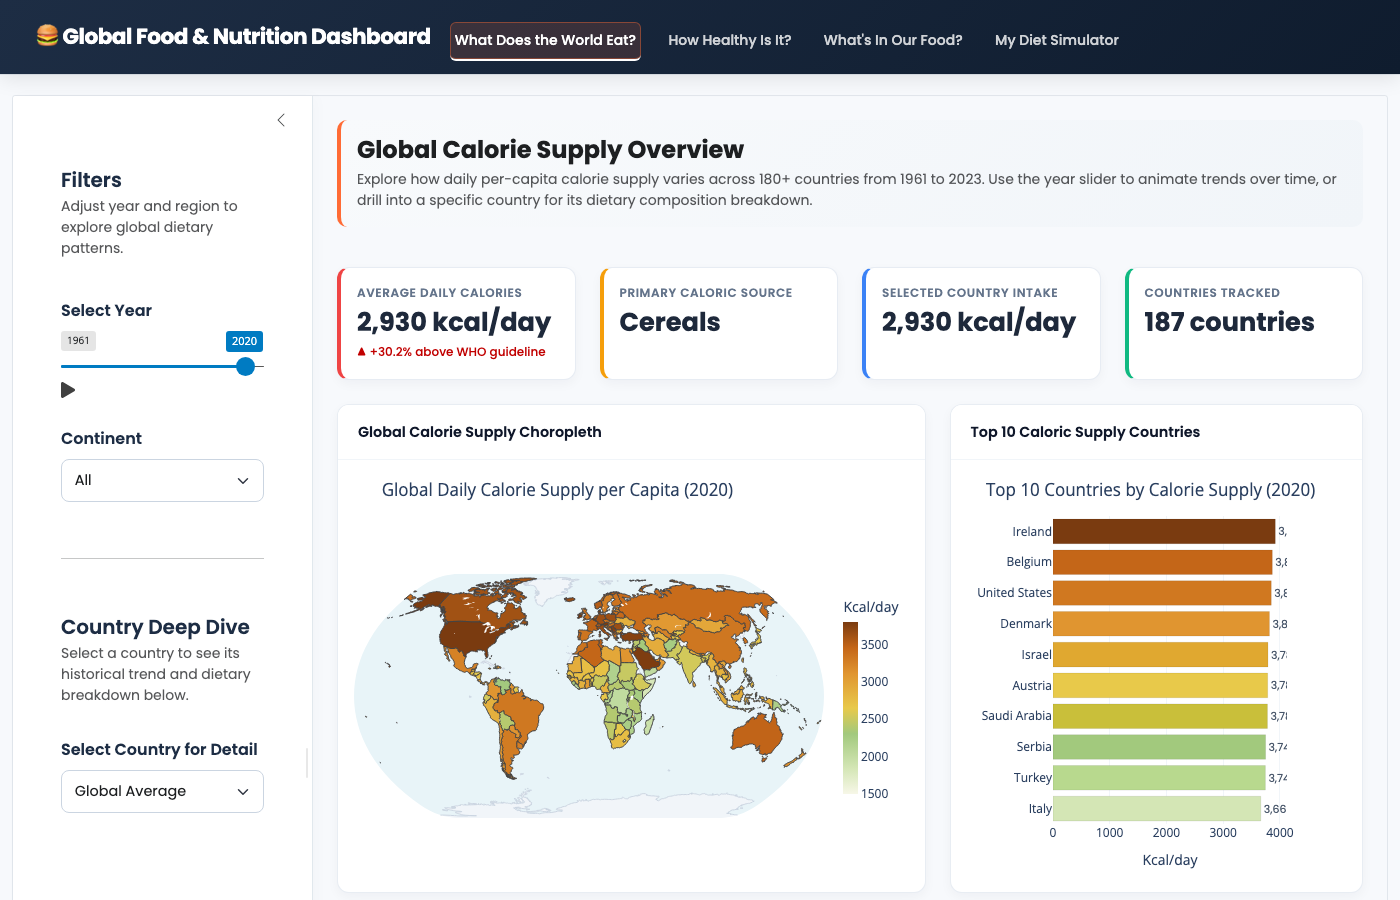
\includegraphics[width=\textwidth,height=0.75\textheight,keepaspectratio]{tab1.png}
    \end{center}
\end{frame}

\begin{frame}{How healthy is it?}
    \begin{center}
        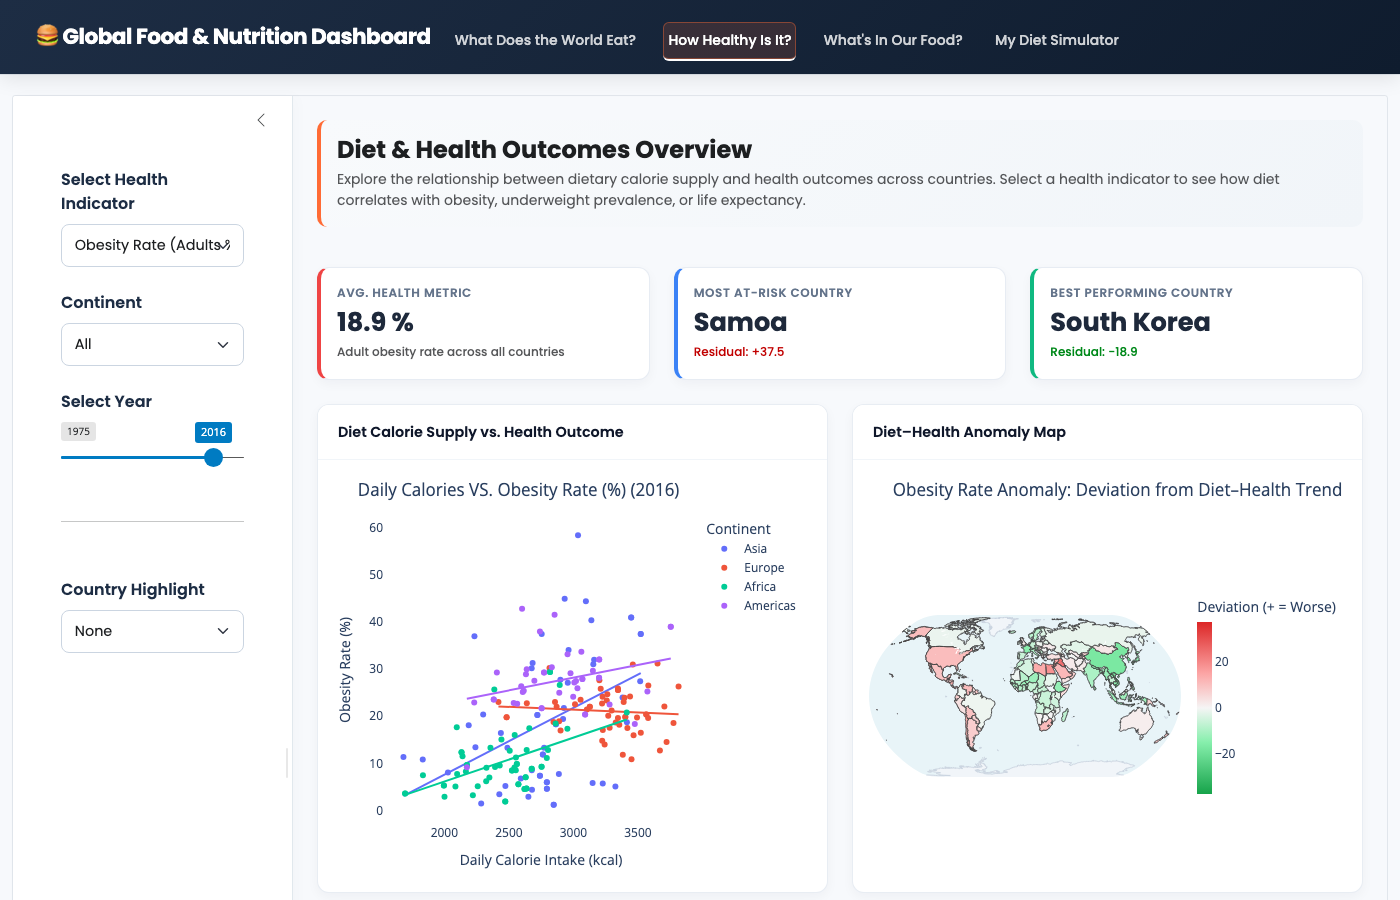
\includegraphics[width=\textwidth,height=0.75\textheight,keepaspectratio]{tab2.png}
    \end{center}
\end{frame}

\begin{frame}{What's in our food?}
    \begin{center}
        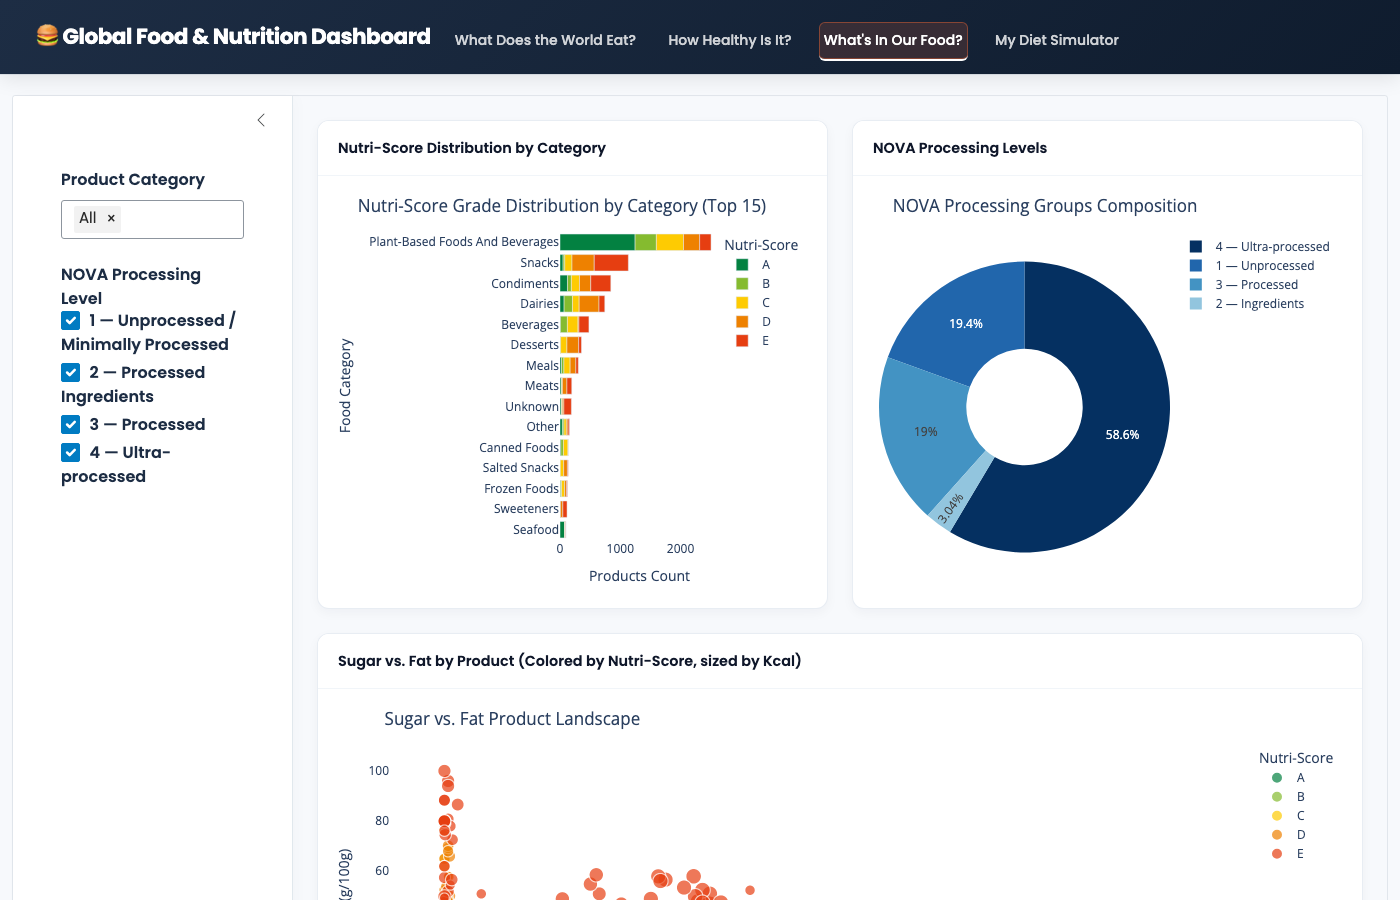
\includegraphics[width=\textwidth,height=0.75\textheight,keepaspectratio]{tab3.png}
    \end{center}
\end{frame}

\begin{frame}{My Diet Simulator}
    \begin{center}
        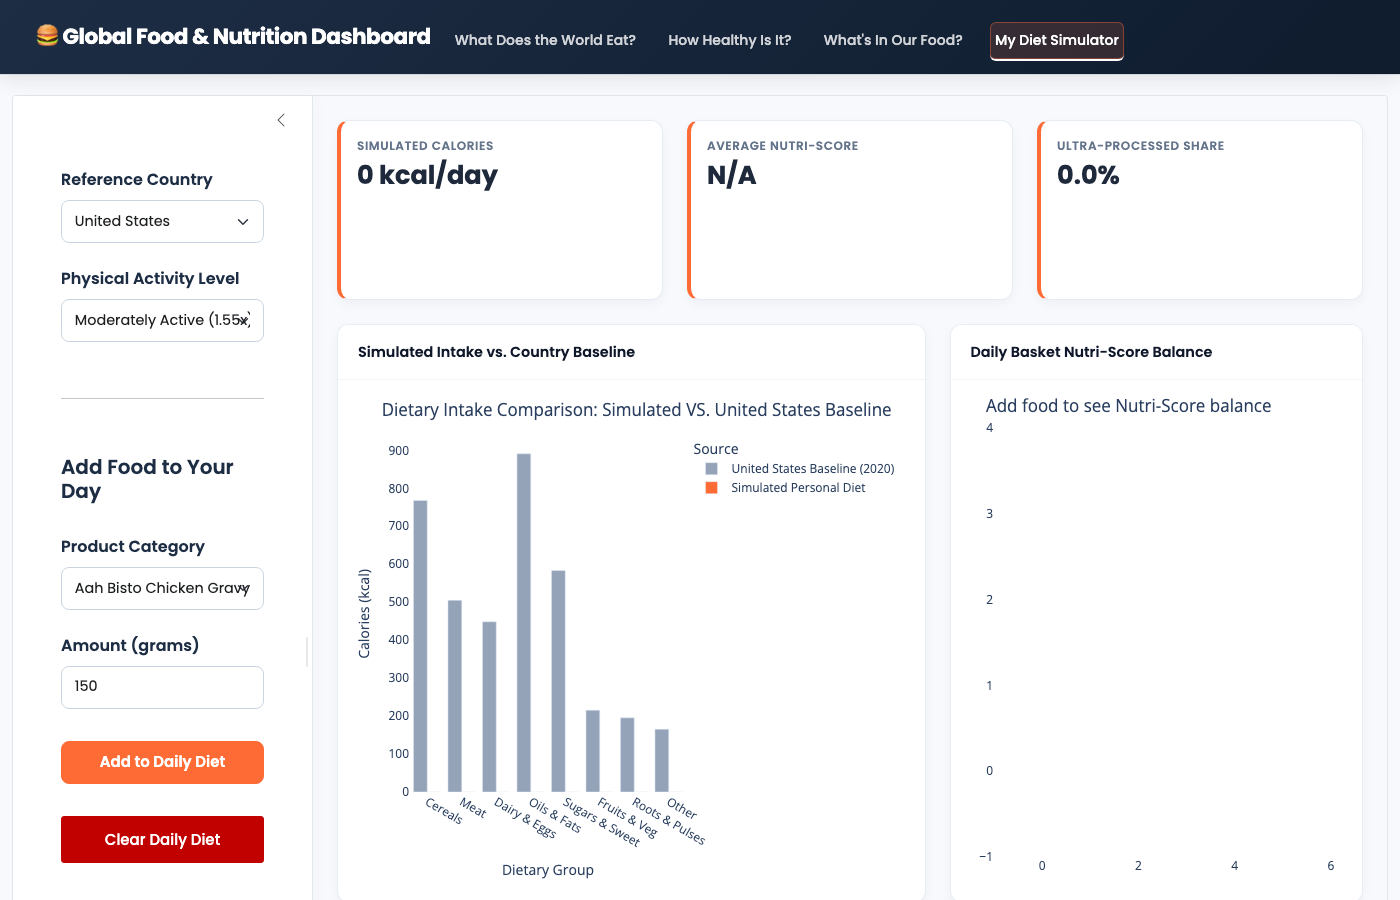
\includegraphics[width=\textwidth,height=0.75\textheight,keepaspectratio]{tab4.png}
    \end{center}
\end{frame}

\section{Findings \& Lessons Learnt}
\begin{frame}{Findings \& Lessons Learnt}
    \textbf{Key Findings:}
    \begin{itemize}
        \item High-calorie diets correlate strongly with obesity, but \textbf{composition} (sugar/fat ratios) is a stronger predictor of health anomalies than total supply alone.
        \item Ultra-processed foods dominate specific categories, heavily impacting average Nutri-Scores.
    \end{itemize}
    
    \vspace{0.3cm}
    \textbf{Lessons Learnt:}
    \begin{itemize}
        \item \textit{Challenge:} Managing Shiny's reactive graph to keep the app performant with tens of thousands of data points.
        \item \textit{Solution:} Effective use of reactive values and selective UI rendering.
    \end{itemize}
\end{frame}

\section{Q \& A}
\begin{frame}{Q \& A}
    \begin{center}
        \Huge \textbf{Thank You!} \\
        \vspace{1cm}
        \large Any Questions?
        
        \vspace{1cm}
        \normalsize \textbf{GitHub Repository:} \\
        \url{https://github.com/miinguyen/global-food-nutrition-dashboard}
    \end{center}
\end{frame}

\end{document}
